\newpage
\problem{2: Remote Sensors} % {10+10+10+20=50}

\problemdes

\begin{figure}[!ht]
    \centering
    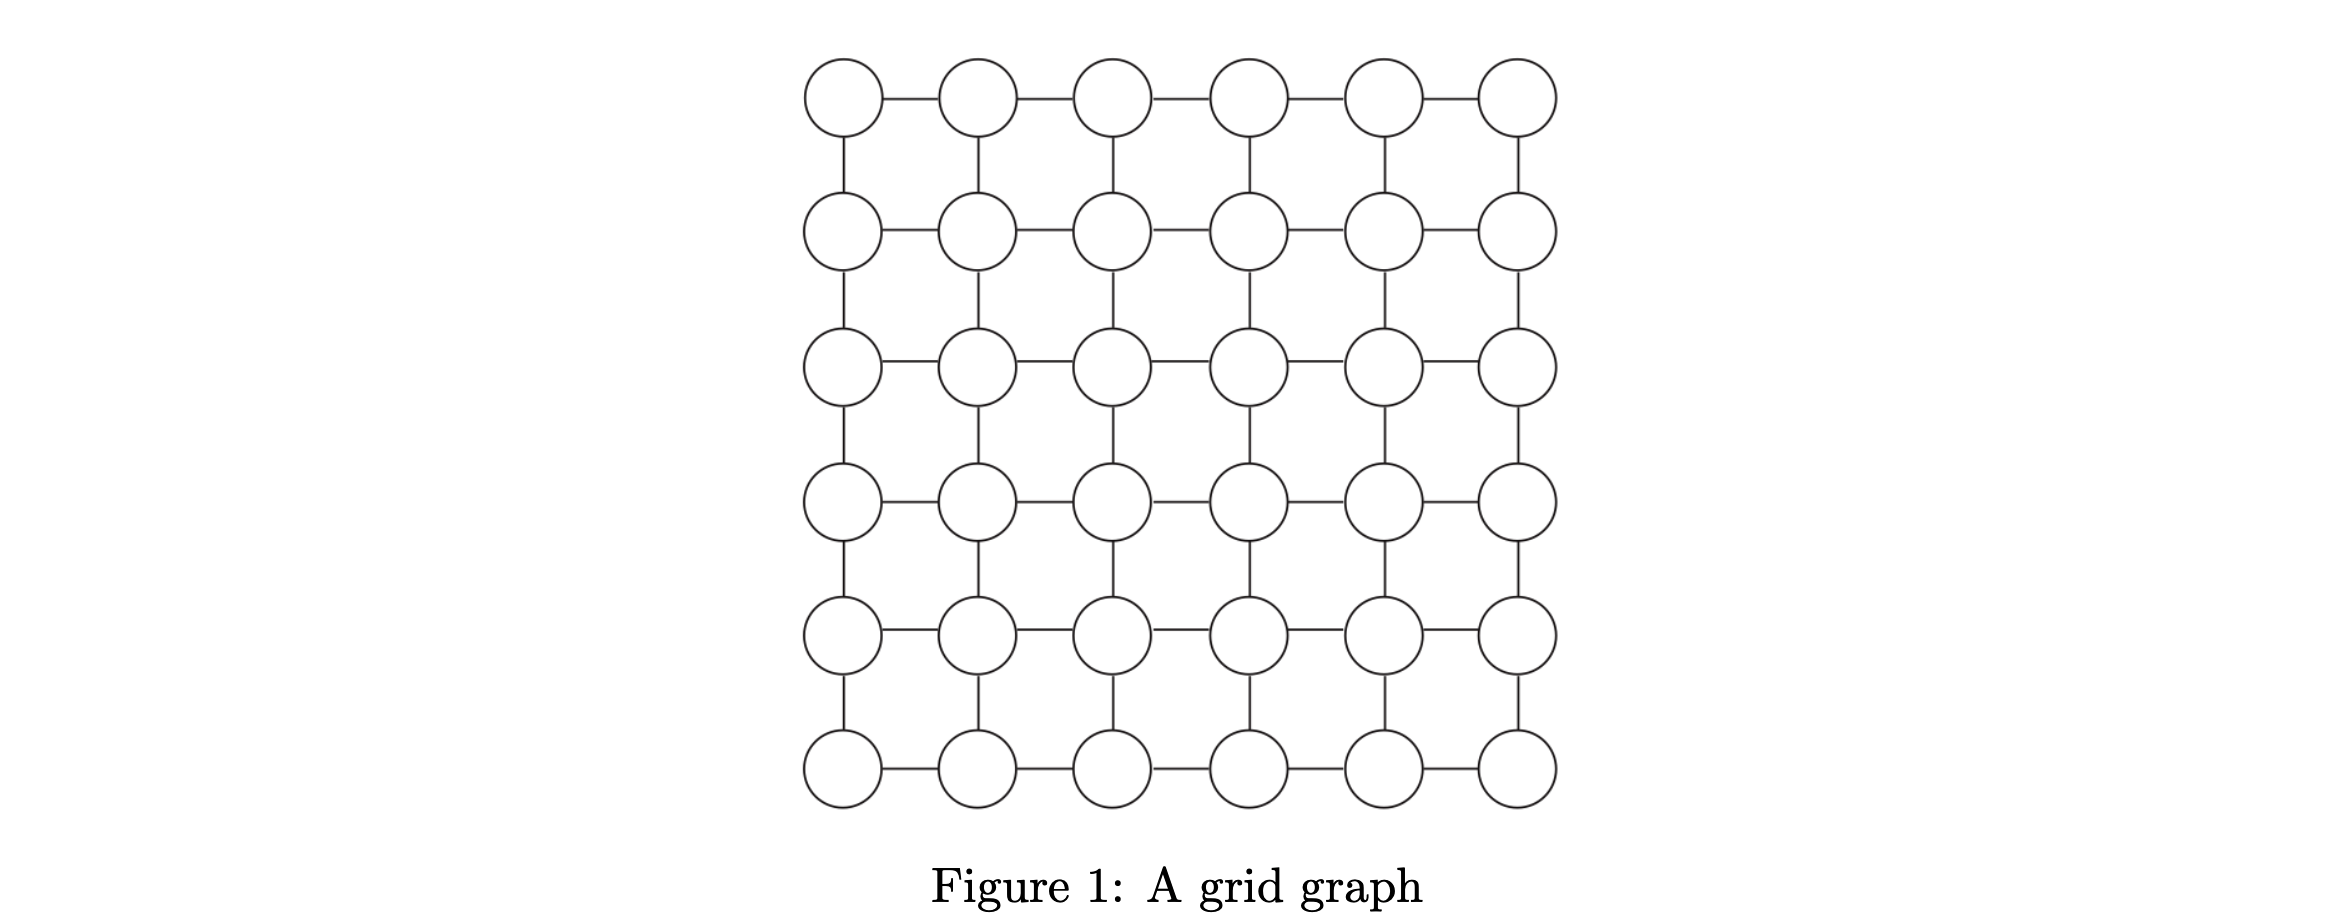
\includegraphics[width=\textwidth]{graph.png}
    \label{fig:algo}
\end{figure}

Suppose you are given an $n \times n$ grid graph $G$, as in Figure 1 Associated with each node $v$ is a weight $w(v)$, which is a nonnegative integer. You may assume that the weights of all nodes are distinct. Your goal is to choose an independent set $S$ of nodes of the grid, so that the sum of the weights of the nodes in $S$ is as large as possible. (The sum of the weights of the nodes in $S$ will be called its total weight.) Consider the following greedy algorithm for this problem.

\begin{figure}[!ht]
    \centering
    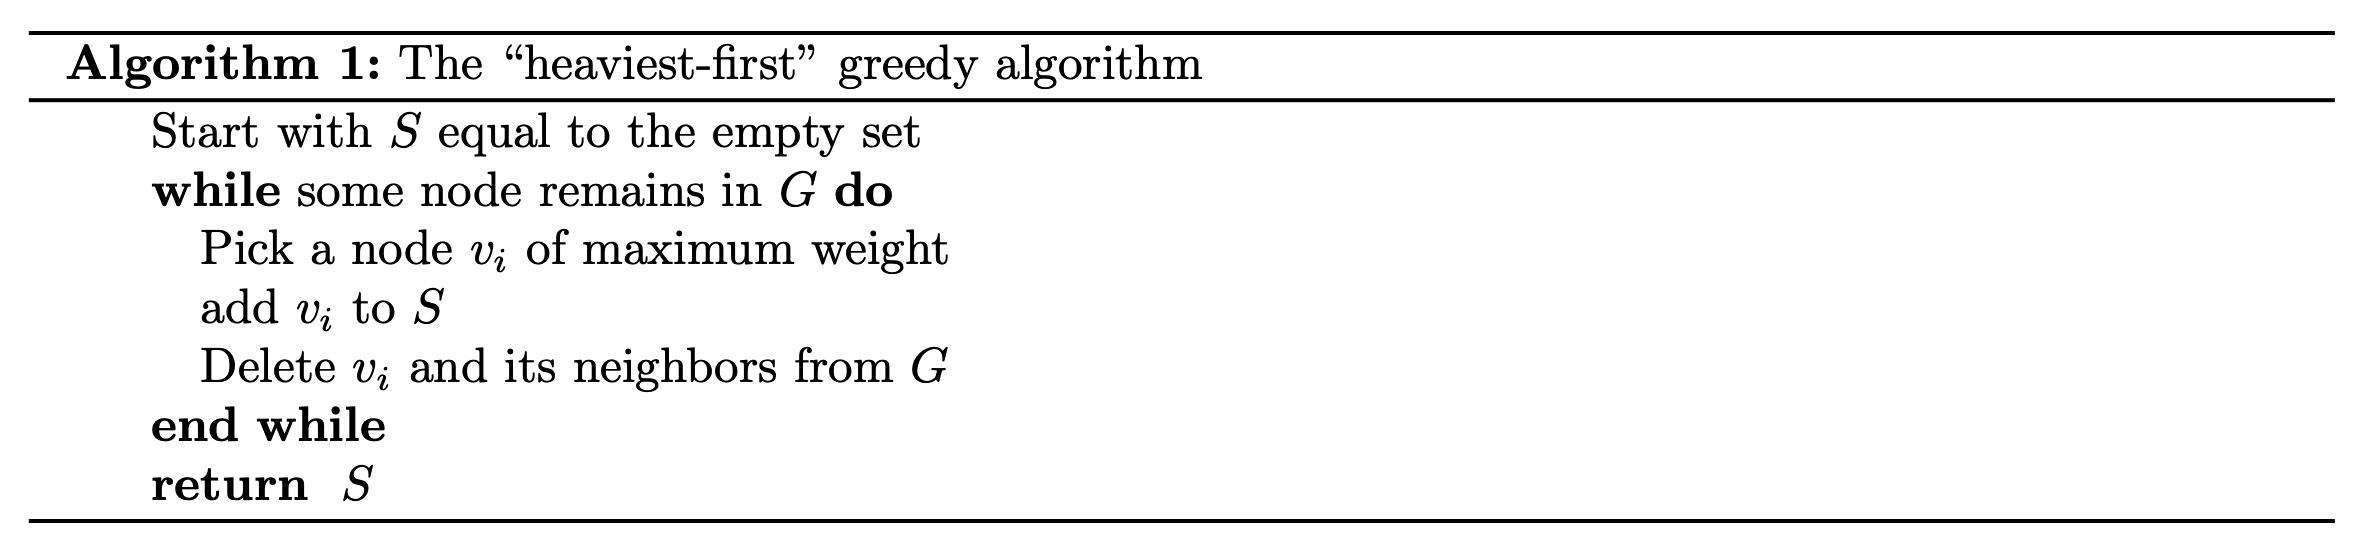
\includegraphics[width=\textwidth]{algorithm.png}
    \label{fig:algo}
\end{figure}

\subproblem{Subproblem 1}

Let $S$ be the independent set returned by the “heaviest-first” greedy algorithm, and let $T$ be any other independent set in $G$. Show that, for each node $v \in T$, either $v \in S$,or there is a node $v' \in S$ so that $w(v) \le w(v\prime)$ and $(v, v\prime)$ is an edge of $G$.

\subsolution{Solution 1}

\subsolution{High-level description}


%\subsolution{Pseudo Code}

\subsolution{Correctness}


\subsolution{Time complexity}




\subproblem{Subproblem 2}

Show that the “heaviest-first” greedy algorithm returns an independent set of total weight at least $1/4$ times the maximum total weight of any independent set in the grid graph $G$.

\subsolution{Solution 2}

\subsolution{High-level description}


%\subsolution{Pseudo Code}

\subsolution{Correctness}


\subsolution{Time complexity}









